
Das Ziel des Visitor-Pattern ist, die Operationen auf Elemente in einer Objektstruktur außerhalb dieser Objektstruktur zu lagern um diese beliebig auszuwechseln.
Die Voraussetzung für jedes Element dieser Objektstruktur ist ein Interface \texttt{Element}, welches eine Methode \texttt{accept(Visitor)} erfordert. Dabei repräsentiert das übergebene Objekt \texttt{Visitor} die Operationen, die auf dieses Element angewendet werden sollen. Der Visitor selbst ist auch ein Interface. Voraussetzung für das Visitor-Pattern ist, dass keine neue Klasse von dem Typ Element hinzugefügt wird, denn das Interface Visitor muss für jeden Typ eine eigene Methode \texttt{visit} implementieren. Das bedeutet für unser UML-Diagramm, mit den zwei verschiedenen Elementen \texttt{ElementA} und \texttt{ElementB}, das wird zwei Methoden \texttt{visitElementA(ElementA)} und \texttt{visitElementB(ElementB)} definieren müssen. 
Der Ablauf des Visitor-Pattern ist dann wie folgt: Zunächst wird einem Element ein konkretes Visitor-Objekt übergeben. Dieses Element ruft dann die für sich implementierte Visit-Methode auf und übergibt sich selbst dem Visitor. Der Visitor kann dann auf das Element zugreifen und es bearbeiten.

\begin{figure}[htbp]
\centering
%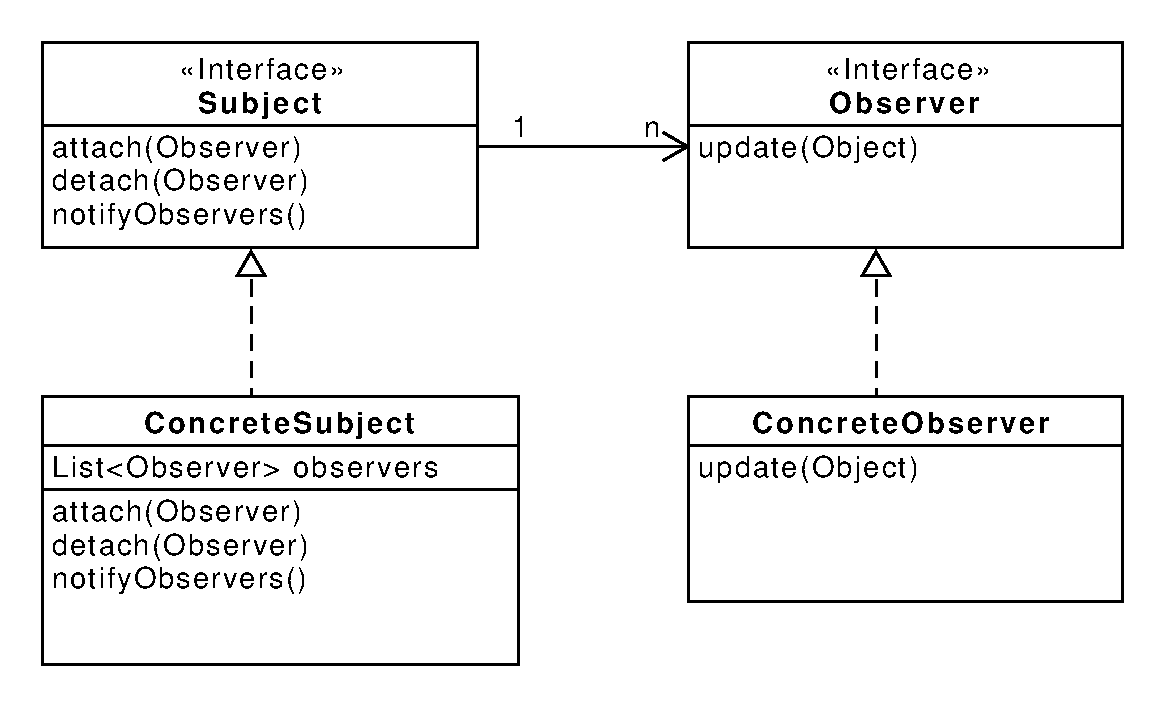
\includegraphics[scale=.5]{./observer/observer}
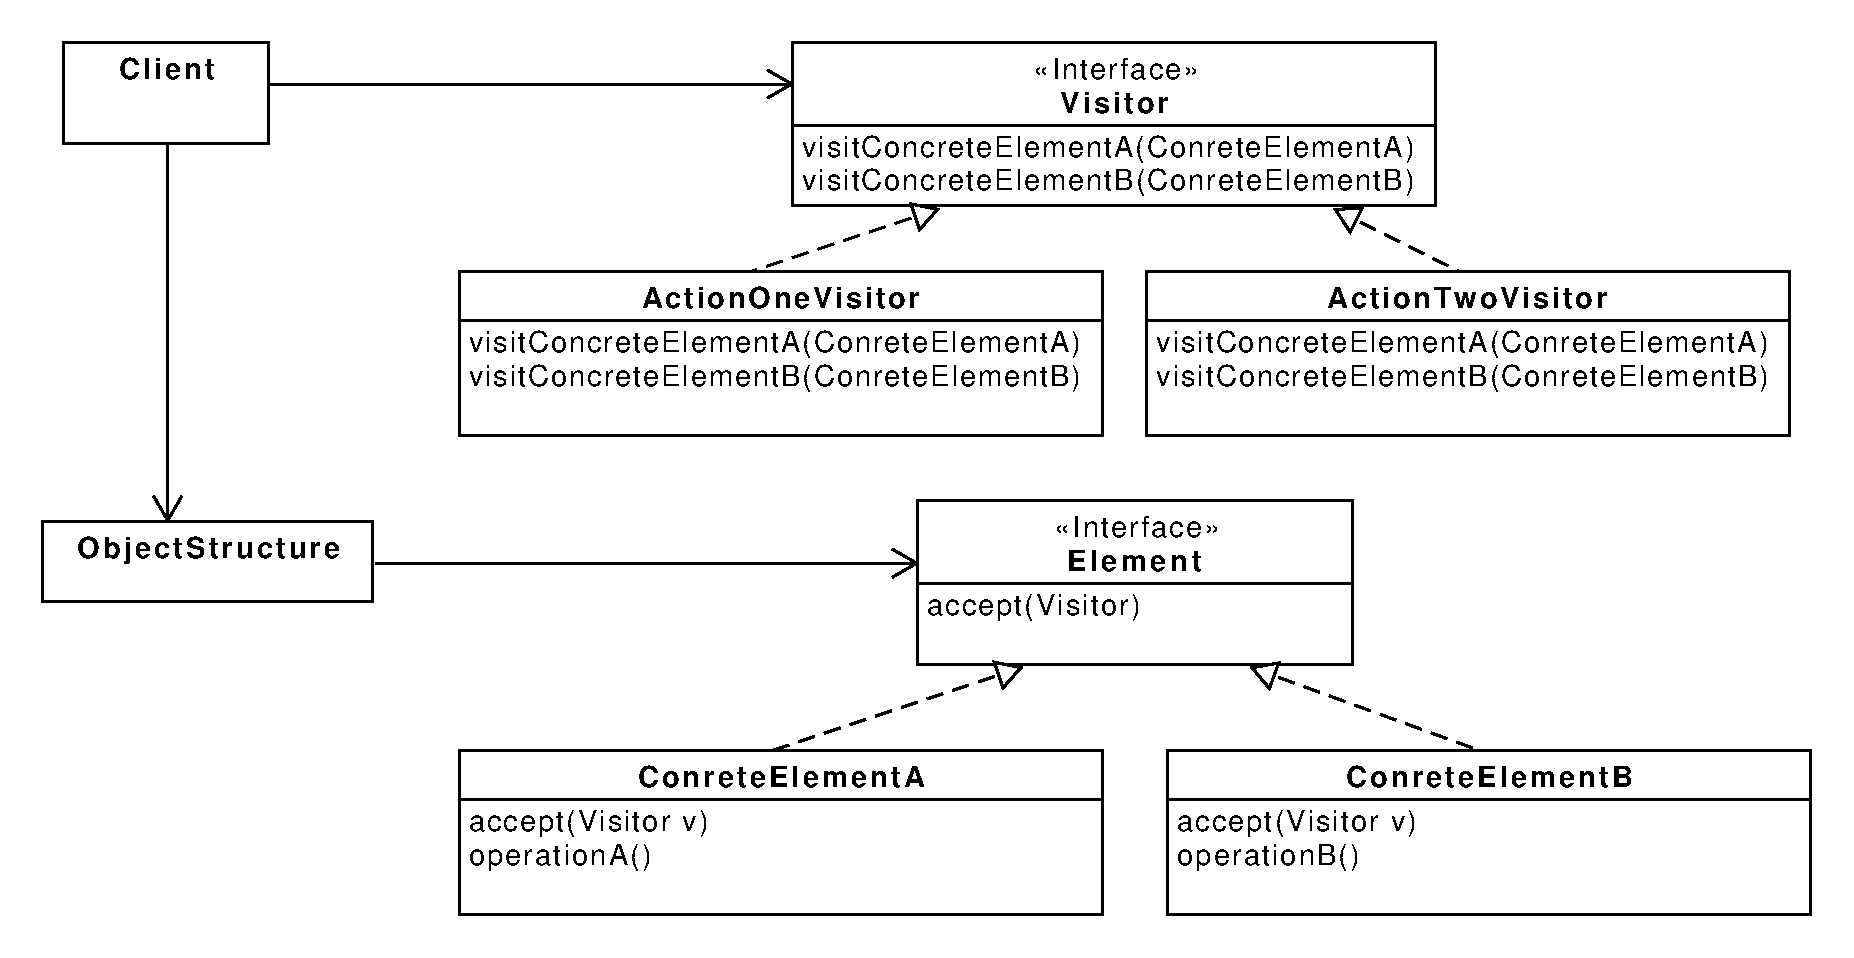
\includegraphics[width=0.9\textwidth]{./paper/visitor/visitor}
\caption{Eine UML-Darstellung von dem Visitor-Pattern.}
\label{visitordiagramm}
\end{figure} 
